\documentclass{article}
\usepackage{geometry}
 \geometry{
 a4paper,
 total={170mm,257mm},
 left=20mm,
 top=20mm,
 }

 \usepackage{caption}
\usepackage[export]{adjustbox} %% for picture frame
\usepackage[english]{babel}
\usepackage[utf8]{inputenc}
\usepackage{fancyhdr}

%%%question enviroment 

%%% Question Environment%%%  use 
%%% Question Environment%%%  use 
%%% Question Environment%%%  use \input{./QueENV.tex}   to include
%% Use \begin{Q}....\end{Q}

\newcounter{QC}
\setcounter{QC}{1}
\newenvironment{Q}[1]{
    \section{Question -\arabic{QC}} \stepcounter{QC}{\large\textbf{#1}}
}

%%% Question Environment%%%

   to include
%% Use \begin{Q}....\end{Q}

\newcounter{QC}
\setcounter{QC}{1}
\newenvironment{Q}[1]{
    \section{Question -\arabic{QC}} \stepcounter{QC}{\large\textbf{#1}}
}

%%% Question Environment%%%

   to include
%% Use \begin{Q}....\end{Q}

\newcounter{QC}
\setcounter{QC}{1}
\newenvironment{Q}[1]{
    \section{Question -\arabic{QC}} \stepcounter{QC}{\large\textbf{#1}}
}

%%% Question Environment%%%



\pagestyle{fancy}
\fancyhf{}
\rhead{\textit{LAB-2}}
\lhead{\textit{Pul074BEX004}}
\rfoot{\thepage}

%%% format and command for lab ans c and assembly

%%% Formating And Command for Embedded Lab   Assambly & C%%%


%%% Formatting And Command for Embedded Lab   Assembly & C%%%
%% 
%%% Formating And Command for Embedded Lab   Assambly & C%%%


%%% Formatting And Command for Embedded Lab   Assembly & C%%%
%% 
%%% Formating And Command for Embedded Lab   Assambly & C%%%


%%% Formatting And Command for Embedded Lab   Assembly & C%%%
%% \input{./asm c.tex}

%% \anscode{problem no. like 1,2,3...}{assembly code file }{ code file}


\usepackage{listings}
\usepackage{multicol}
\usepackage{mdframed}

\renewcommand{\lstlistlistingname}{List of Codes}
\renewcommand{\lstlistingname}{Code}


\setlength{\columnsep}{0.5cm}

\usepackage{xcolor}
\definecolor{codegreen}{rgb}{0,0.6,0}
\definecolor{codegray}{rgb}{0.4,0.4,0.4}
\definecolor{codepurple}{rgb}{0.58,0,0.82}
%\definecolor{backcolour}{rgb}{0.95,0.99,0.92}
\definecolor{backcolour}{rgb}{0,0,0}


\lstdefinestyle{customa}{
  backgroundcolor=\color{backcolour},   commentstyle=\color{codegreen},
  keywordstyle=\color{magenta},
  numberstyle=\tiny\color{codegray},
  stringstyle=\color{codepurple},
  basicstyle=\ttfamily\small\color{white},
  breakatwhitespace=false,
  breaklines=true,
  captionpos=b,
  morekeywords={MOV,ADD,ADDC,ACALL,INC,DJNZ,AJMP,RET,END,ORG,RR,JNC,SUBB,JC,DEC,ANL,SWAP,MUL,DIV,CLR,SETB},
  keepspaces=true,
  numbers=left,
  numbersep=5pt,
  showspaces=false,
  showstringspaces=false,
  showtabs=false,
  tabsize=4
}

\lstdefinestyle{customc}{
  backgroundcolor=\color{backcolour},   commentstyle=\color{codegreen},
  keywordstyle=\color{cyan},
  numberstyle=\tiny\color{codegray},
  stringstyle=\color{codepurple},
  basicstyle=\ttfamily\footnotesize\color{white},
  breakatwhitespace=false,
  breaklines=true,
  captionpos=b,
  keepspaces=true,
  language=C,
  numbers=left,
  numbersep=5pt,
  showspaces=false,
  showstringspaces=false,
  showtabs=false,
  tabsize=3
}




\newcommand {\anscode}[3]{

  \begin{center}
    \textbf{Assembly}
  \end{center}

  \begin{multicols}{2}
    \lstinputlisting[style=customa,nolol]{#2}
  \end{multicols}

  \begingroup
  \captionof{lstlisting}{Problem no. #1 Assembly}
  \endgroup


  \vspace{2 em}


  \begin{center}
    \textbf{C language }
  \end{center}
  \begin{multicols}{2}
    \lstinputlisting[style=customc,nolol]{#3}
  \end{multicols}

  \begingroup
  \captionof{lstlisting}{Problem no. #1 C language}
  \endgroup
}

%%% Formating And Command for Embedded Lab  Assambly & C%%%

%% \anscode{problem no. like 1,2,3...}{assembly code file }{ code file}


\usepackage{listings}
\usepackage{multicol}
\usepackage{mdframed}

\renewcommand{\lstlistlistingname}{List of Codes}
\renewcommand{\lstlistingname}{Code}


\setlength{\columnsep}{0.5cm}

\usepackage{xcolor}
\definecolor{codegreen}{rgb}{0,0.6,0}
\definecolor{codegray}{rgb}{0.4,0.4,0.4}
\definecolor{codepurple}{rgb}{0.58,0,0.82}
%\definecolor{backcolour}{rgb}{0.95,0.99,0.92}
\definecolor{backcolour}{rgb}{0,0,0}


\lstdefinestyle{customa}{
  backgroundcolor=\color{backcolour},   commentstyle=\color{codegreen},
  keywordstyle=\color{magenta},
  numberstyle=\tiny\color{codegray},
  stringstyle=\color{codepurple},
  basicstyle=\ttfamily\small\color{white},
  breakatwhitespace=false,
  breaklines=true,
  captionpos=b,
  morekeywords={MOV,ADD,ADDC,ACALL,INC,DJNZ,AJMP,RET,END,ORG,RR,JNC,SUBB,JC,DEC,ANL,SWAP,MUL,DIV,CLR,SETB},
  keepspaces=true,
  numbers=left,
  numbersep=5pt,
  showspaces=false,
  showstringspaces=false,
  showtabs=false,
  tabsize=4
}

\lstdefinestyle{customc}{
  backgroundcolor=\color{backcolour},   commentstyle=\color{codegreen},
  keywordstyle=\color{cyan},
  numberstyle=\tiny\color{codegray},
  stringstyle=\color{codepurple},
  basicstyle=\ttfamily\footnotesize\color{white},
  breakatwhitespace=false,
  breaklines=true,
  captionpos=b,
  keepspaces=true,
  language=C,
  numbers=left,
  numbersep=5pt,
  showspaces=false,
  showstringspaces=false,
  showtabs=false,
  tabsize=3
}




\newcommand {\anscode}[3]{

  \begin{center}
    \textbf{Assembly}
  \end{center}

  \begin{multicols}{2}
    \lstinputlisting[style=customa,nolol]{#2}
  \end{multicols}

  \begingroup
  \captionof{lstlisting}{Problem no. #1 Assembly}
  \endgroup


  \vspace{2 em}


  \begin{center}
    \textbf{C language }
  \end{center}
  \begin{multicols}{2}
    \lstinputlisting[style=customc,nolol]{#3}
  \end{multicols}

  \begingroup
  \captionof{lstlisting}{Problem no. #1 C language}
  \endgroup
}

%%% Formating And Command for Embedded Lab  Assambly & C%%%

%% \anscode{problem no. like 1,2,3...}{assembly code file }{ code file}


\usepackage{listings}
\usepackage{multicol}
\usepackage{mdframed}

\renewcommand{\lstlistlistingname}{List of Codes}
\renewcommand{\lstlistingname}{Code}


\setlength{\columnsep}{0.5cm}

\usepackage{xcolor}
\definecolor{codegreen}{rgb}{0,0.6,0}
\definecolor{codegray}{rgb}{0.4,0.4,0.4}
\definecolor{codepurple}{rgb}{0.58,0,0.82}
%\definecolor{backcolour}{rgb}{0.95,0.99,0.92}
\definecolor{backcolour}{rgb}{0,0,0}


\lstdefinestyle{customa}{
  backgroundcolor=\color{backcolour},   commentstyle=\color{codegreen},
  keywordstyle=\color{magenta},
  numberstyle=\tiny\color{codegray},
  stringstyle=\color{codepurple},
  basicstyle=\ttfamily\small\color{white},
  breakatwhitespace=false,
  breaklines=true,
  captionpos=b,
  morekeywords={MOV,ADD,ADDC,ACALL,INC,DJNZ,AJMP,RET,END,ORG,RR,JNC,SUBB,JC,DEC,ANL,SWAP,MUL,DIV,CLR,SETB},
  keepspaces=true,
  numbers=left,
  numbersep=5pt,
  showspaces=false,
  showstringspaces=false,
  showtabs=false,
  tabsize=4
}

\lstdefinestyle{customc}{
  backgroundcolor=\color{backcolour},   commentstyle=\color{codegreen},
  keywordstyle=\color{cyan},
  numberstyle=\tiny\color{codegray},
  stringstyle=\color{codepurple},
  basicstyle=\ttfamily\footnotesize\color{white},
  breakatwhitespace=false,
  breaklines=true,
  captionpos=b,
  keepspaces=true,
  language=C,
  numbers=left,
  numbersep=5pt,
  showspaces=false,
  showstringspaces=false,
  showtabs=false,
  tabsize=3
}




\newcommand {\anscode}[3]{

  \begin{center}
    \textbf{Assembly}
  \end{center}

  \begin{multicols}{2}
    \lstinputlisting[style=customa,nolol]{#2}
  \end{multicols}

  \begingroup
  \captionof{lstlisting}{Problem no. #1 Assembly}
  \endgroup


  \vspace{2 em}


  \begin{center}
    \textbf{C language }
  \end{center}
  \begin{multicols}{2}
    \lstinputlisting[style=customc,nolol]{#3}
  \end{multicols}

  \begingroup
  \captionof{lstlisting}{Problem no. #1 C language}
  \endgroup
}

%%% Formating And Command for Embedded Lab  Assambly & C%%%
%%%%>>>>>>>........
%%%%%% include  Titles.%%%% use \input{./CP}%%%
%%%use """"""""    \CP{}{}{}{}   """" %%%% and 4 argument to craete Title page 
%%%%%%%%%%%%%%%%%%%%%%%%%%%%%%%%%%%%%%%%%%%%%%%%%%%%%%%%%%%%%%%%%
%%%argument number
%% 1=major header ## Course name 
%% 2=minor4 heading ## lab/assignmet no
%% 3=Title  ## Assignment or Lab title
%% 4=submitted to::## input receiver Name"
%%%%%%%%%%%%%%%%%%%%%%%%%%%%%%%%%%%%%%%%%%%%%%%%%%%%%%%%%%%%%%%%%


\usepackage{mathpazo} % Palatino font
\usepackage{graphicx}
\usepackage{float}

%%% format and command for lab ans c and assembly

\newcommand{\HRule}{\rule{\linewidth}{0.4mm}} % Defines a new command for horizontal lines, change thickness here



%----------------------------------------------------------------------------------------
%	TITLE PAGE
%----------------------------------------------------------------------------------------


\newcommand{\CP}[4]{ \begin{titlepage} % Suppresses displaying the page number on the title page and the subsequent page counts as page 1
		%%%%  univerdity logo%%
		\begin{figure}[H]
			\centering
			
\includegraphics[scale=0.13]{tulogo.jpg}
		\end{figure}
		%%% end university logo

		\center % Centre everything on the page

		%------------------------------------------------
		%	Headings
		%------------------------------------------------

		\textsc{\huge Institute of Engineering \\ Central Campus,Pulchowk}\\[1.5cm] % Main heading such as the name of your university/college

		\textsc{\Large #1}\\[0.5cm] % Major heading such as course name

		\textsc{\large #2}\\[0.5cm] % Minor heading such as assignment no./ lab no.

		%------------------------------------------------
		%	Title
		%------------------------------------------------

		\HRule\\[0.4cm]

		{\Huge\bfseries #3}\\[0.4cm] % Title of your document

		\HRule\\[1.5cm]

		%------------------------------------------------
		%	Author(s)
		%------------------------------------------------
		\vfill\vfill
		\begin{minipage}{0.4\textwidth}
			\begin{flushleft}
				\large{
				\textbf{Submitted BY:}\\
				{\normalsize AMRIT PRASAD PHUYAL}\\ % NAME
				{\normalsize Roll: PULL074BEX004}} % Roll
			\end{flushleft}
		\end{minipage}
		~
		\begin{minipage}{0.4\textwidth}
			\begin{flushright}
				\large
				\textbf{Submitted To:}\\
				{ \normalsize{#4}\\ }% recepent's  Name 
				{\normalsize Department of Electronics and Computer Engineering}
			\end{flushright}
		\end{minipage}

		%------------------------------------------------
		%	Date
		%------------------------------------------------

		\vfill\vfill\vfill % Position the date 3/4 down the remaining page

		{\large\today} % Date, change the \today to a set date if you want to be precise

		\vfill % Push the date up 1/4 of the remaining page

	\end{titlepage}
}

\begin{document}

%----------------------------------------------------------------------------------------
%	TITLE PAGE
%----------------------------------------------------------------------------------------
\CP{Embedded system}{LAB \#2}
{Interfacing 7-Segment LED Display with 8051/8052 Micro-controller}
{Department of Electronics and Computer Engineering}




%----------------------------------------------------------------------------------------
\pagenumbering{gobble}
\tableofcontents
\pagebreak
\listoffigures
\pagebreak
\lstlistoflistings
\pagebreak
\pagenumbering{arabic}
\section{Introduction}
\subsection{Microcontroller}

A microcontroller is an integrated circuit ( IC), usually via an MPU, memory and certain peripherals, to control other parts of an electronic system .
These devices are optimized for embed-in applications that require agile and agile processing, digital, analog or electromechanical interactions.
\subsection{8051 Microcontroller}
In 1981, Intel introduced an 8-bit microcontroller called the 8051. It was referred as system on a chip because it had 128 bytes of RAM, 4K byte of on-chip ROM,
two timers, one serial port, and 4 ports (8-bit wide), all on a single chip.\\\\
The different features of the 8051 microcontroller include:
\begin{itemize}
  \item 4KB bytes on-chip program memory (ROM)
  \item 128 bytes on-chip data memory (RAM)
  \item Four register banks
  \item 128 user defined software flags
  \item 8-bit bidirectional data bus
  \item 16-bit unidirectional address bus
  \item 32 general purpose registers each of 8-bit
  \item 16 bit Timers (usually 2, but may have more or less)
  \item Three internal and two external Interrupts
  \item Four 8-bit ports,(short model have two 8-bit ports)
  \item 16-bit program counter and data pointer
  \item 8051 may also have a number of special features such as UARTs, ADC, Op-amp, etc.
\end{itemize}
\begin{figure}[H]
  \centering
  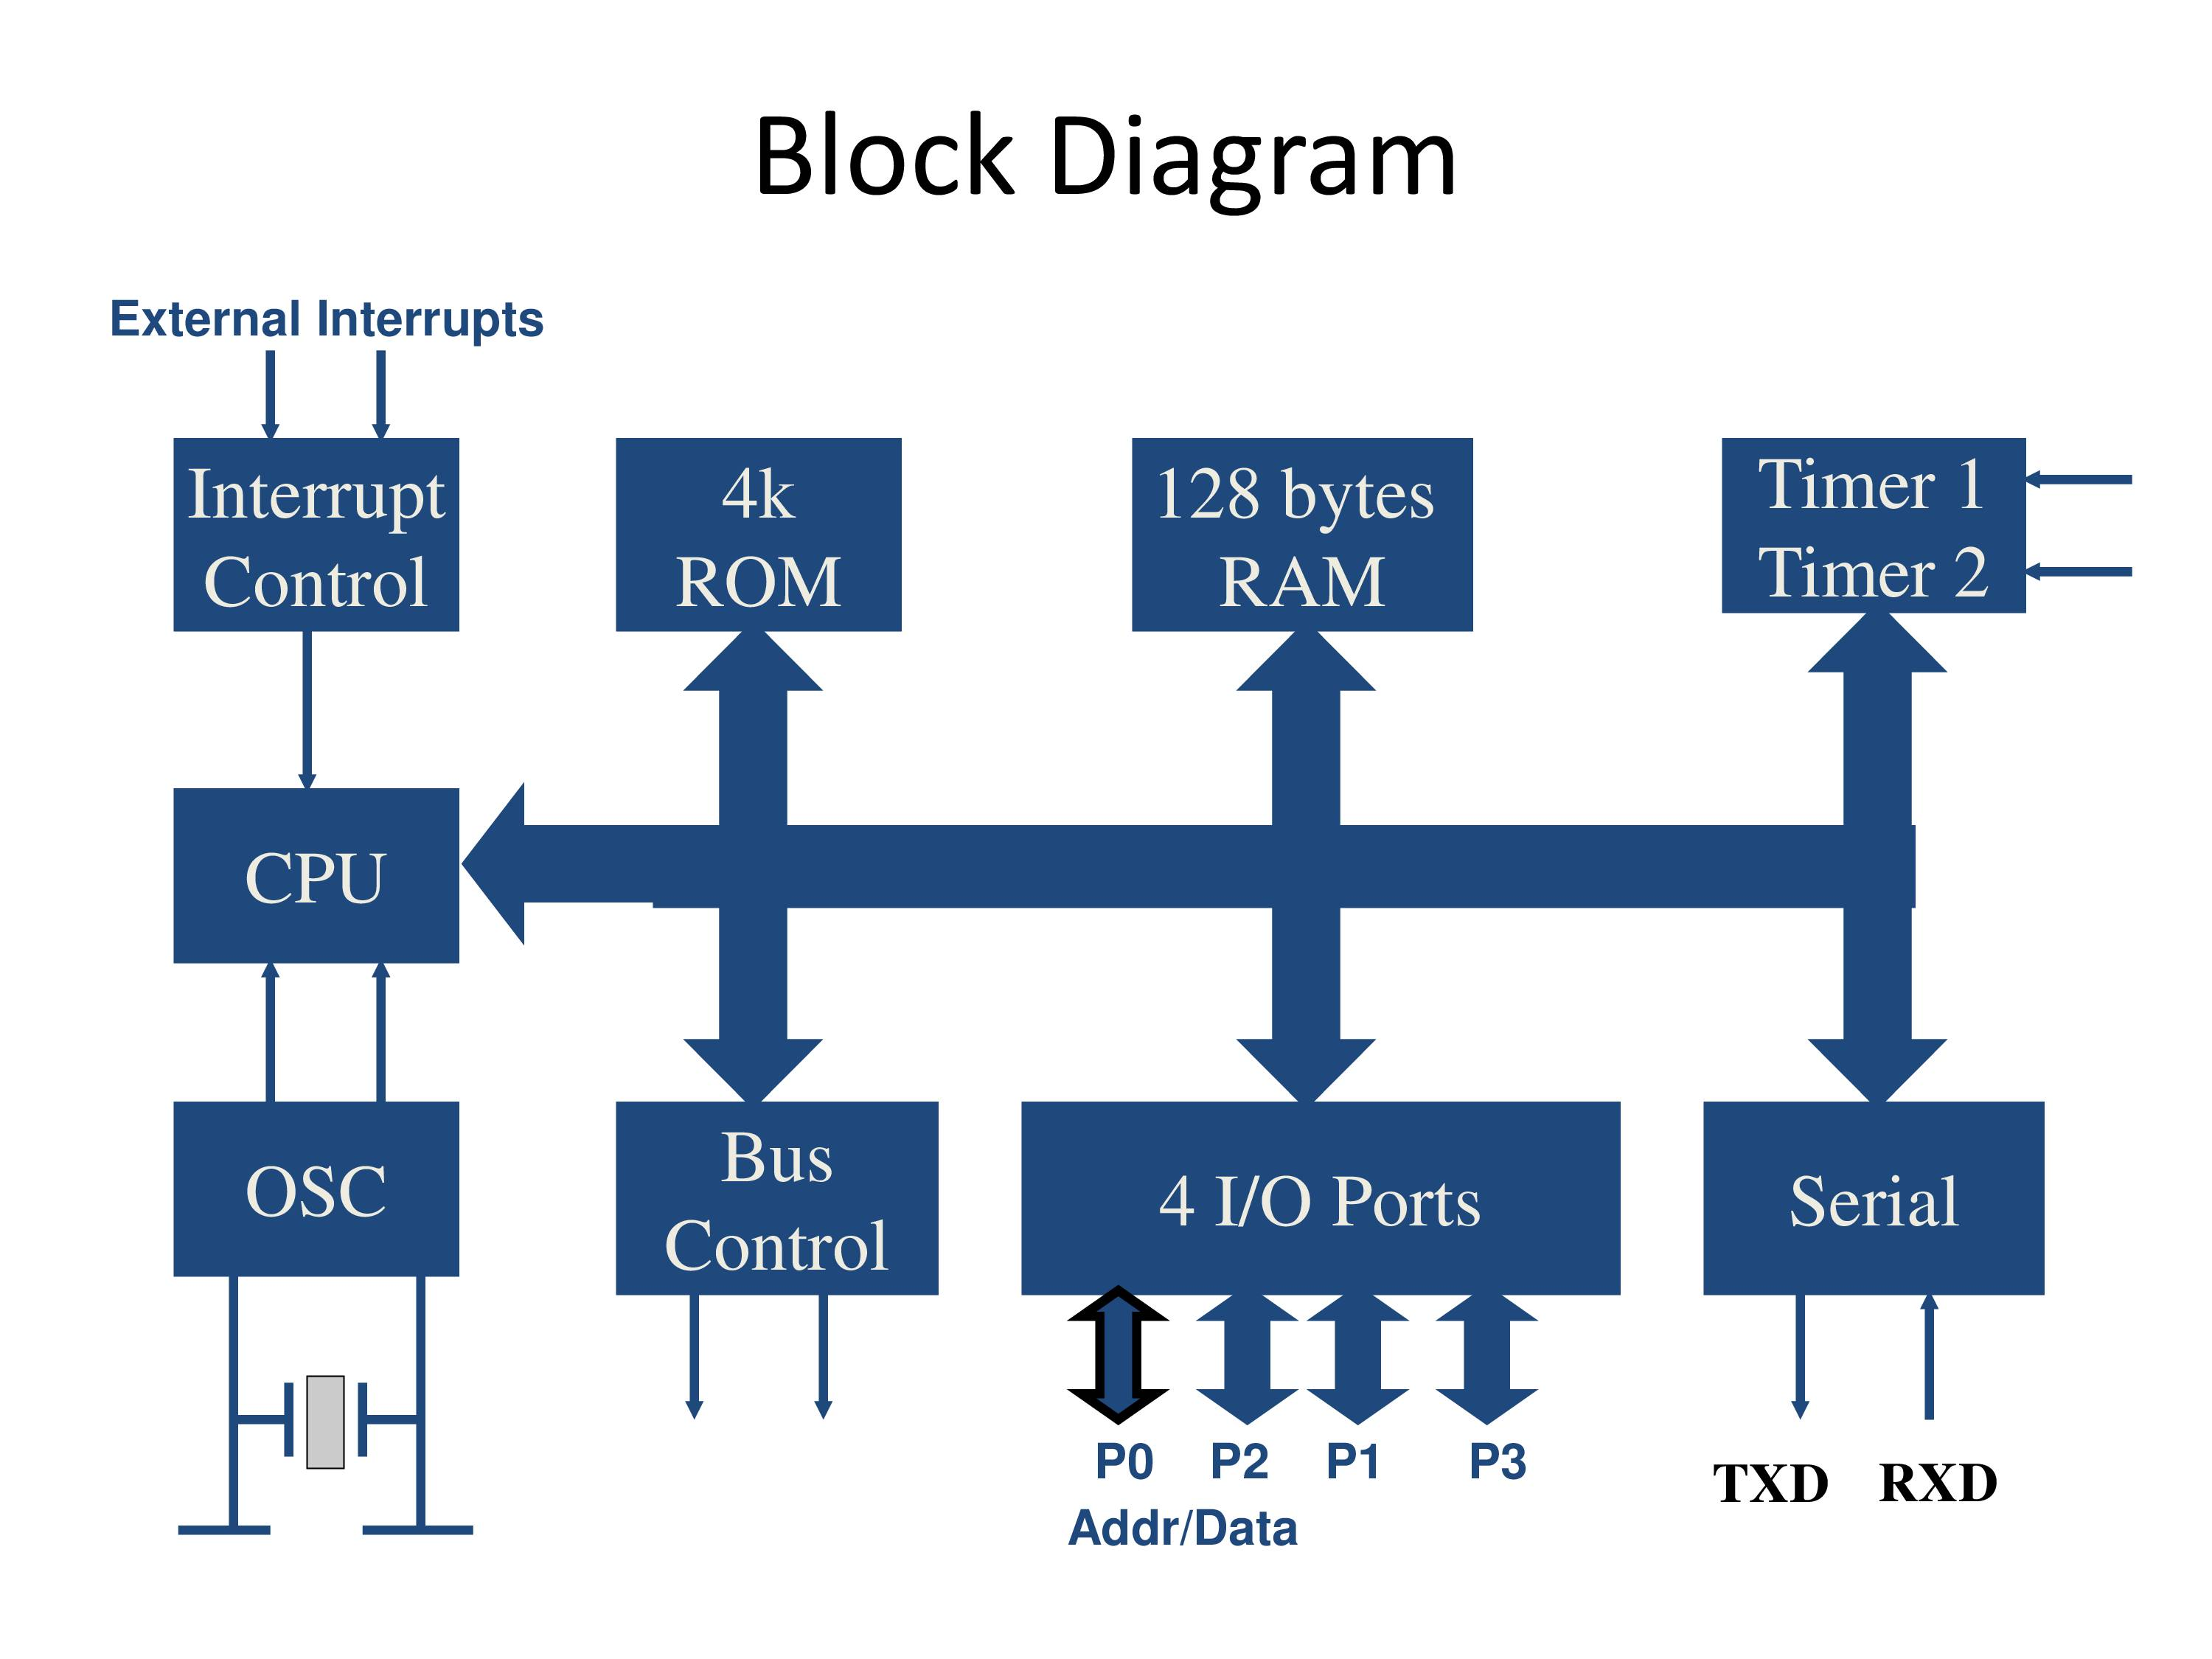
\includegraphics[scale=0.52,cframe=blue 0.5pt 3pt]{./block_diagram.jpg}
  \textit{\caption{Block diagram of 8051 microcontroller}}

\end{figure}

\subsection{7-Segment LED Display}
A seven segment display module is an electronic device used to display digital numbers and
it is made up of seven LED segments. LEDs are PN-junction diodes which emit energy by a process called electroluminescence.
Because of the small size of the LEDs, it is really easy for a number of them to be connected together to make a unit like seven segment display.
The light energy is emitted as ‘photons’ when it is forward biased by a voltage applied across its junctions.
In a seven segment display module, seven LED s are arranged in a rectangle. Sometimes,
an additional LED is seen in a seven segment display unit which is meant for displaying a decimal point.

Features of seven segment Display:-

\begin{itemize}
  \item Available in two modes Common Cathode (CC) and Common Anode (CA)
  \item Available in many different sizes like 9.14mm,14.20mm,20.40mm,38.10mm,57.0mm and 100mm (Commonly used/available size is 14.20mm)
  \item Available colours: White, Blue, Red, Yellow and Green (Res is commonly used)
  \item Low current operation
  \item Better, brighter and larger display than conventional LCD displays.
  \item Current consumption : 30mA / segment
  \item Peak current : 70mA
\end{itemize}

The displays common pin is generally used to identify which type of 7-segment display it is. As each LED has two connecting pins,
one called the “Anode” and the other called the “Cathode”, there are therefore two types of LED 7-segment display called: Common Cathode (CC) and Common Anode (CA).
The difference between the two displays, as their name suggests,
is that the common cathode has all the cathodes of the 7-segments connected directly together and the common anode has all the anodes of the 7-segments connected together
\begin{figure}[H]
  \centering
  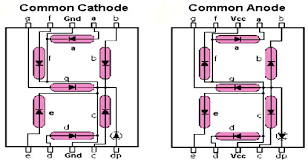
\includegraphics[scale=1.1,cframe=blue 0.5pt 3pt]{./Common cathode vs common anode.png}
  \textit{\caption{Common cathode vs Common anode 7 segment display}}
\end{figure}


\begin{figure}[H]
  \centering
  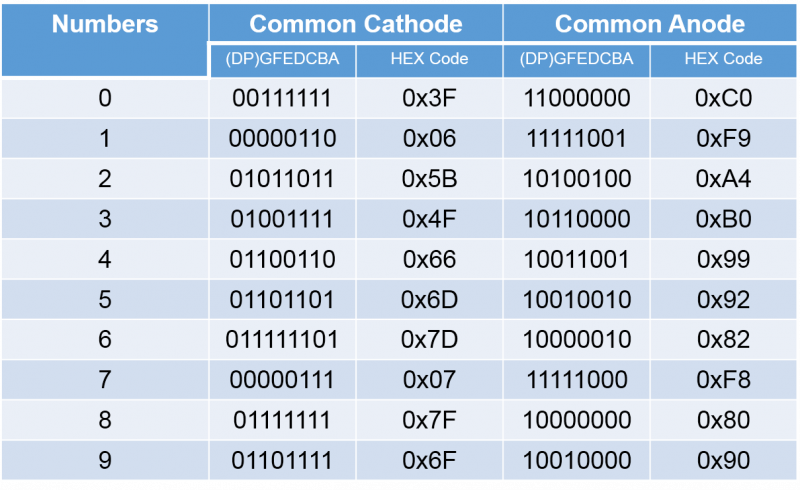
\includegraphics[scale=0.65,cframe=blue 0.5pt 3pt]{./Dispaly codes.png}
  \textit{\caption{Lookup table for Common anode and Common Cathode}}
\end{figure}

\subsection{Applications}
\begin{itemize}
  \item Used in applications where font size is required to be bigger
  \item Microcontroller Independent, hence used in small circuit projects
  \item Used in combination with four segments to display measurement/sensor value  with four characters
  \item Has bright illumination, hence used where display are required to work in low light or dark conditions
\end{itemize}

\section{Objective}
To enable us to write assembly language code for the 8051/8052 micro-controller capable of:
\begin{itemize}
  \item Displaying non-multiplexed and multiplexed output on 7-segment LED units
  \item Displaying static and scrolling output on 7-segment LED units
\end{itemize}

\section{Equipment Required }
\begin{itemize}
  \item Hardware:  8051 or 8052 micro-controller development board, Jumper cables
  \item Simulation Software: KEIL, Vision-Embedded development tool, Proteus Design Suite – Professional PCB layout,
        circuit design and simulation tool
  \item In-System Programming (ISP) Software: ProgISP – An in-system-programmable tool to load HEX  files in to micro-controller
  \item Device Drivers: LibUSB – Application controlling data transfer to/from USB devices
\end{itemize}

\section{Circuit Description }
The circuit diagram, consisting of micro-controller AT89C52 and four common cathode 7 segment display,
used for simulation for this lab is shown below:
\begin{figure}
  \centering
  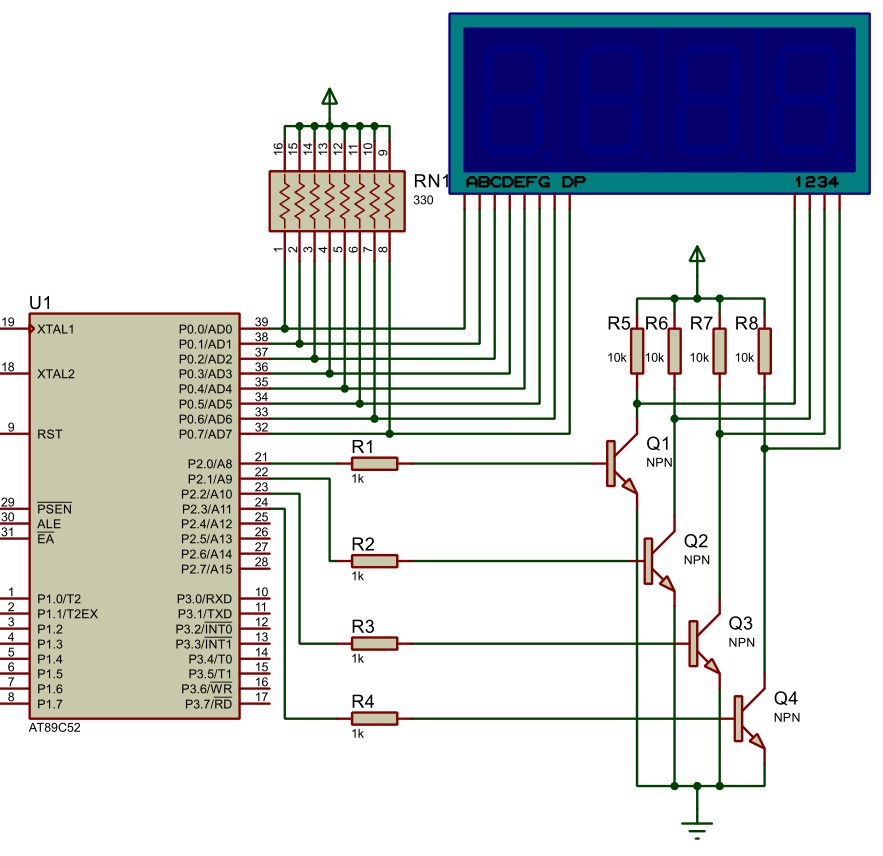
\includegraphics[scale=0.6,cframe=blue 0.5pt 3pt]{./circuit.jpg}
  \textit{\caption{Circuit for Proteus Simulation}}
\end{figure}


Figure shows that the common data lines, from the array of four seven segment display,
are connected to the PORT 0 of microcontroller with array of 8 pull-up resistor.
Here data line A is connected to P0.0 (LSB) whereas DP is connected to P0.7 (MSB).
The control pins 1, 2, 3 and 4 are indirectly connected to P2.0, P2.1, P2.2 and P2.3 respectively.
Since logic low should be applied to control pin to trigger corresponding segment,
here transistor is used to invert the logic. It means in order to trigger a certain segment, let’s say 1,
logic high is applied to the connected pin, here P2.0,
so that there will be logic low across the transistor where the control pin 1 is connected.


Now in order to display digits on more than one segment then illusion technique most be used.
It means we have to give an illusion that multiple values are displayed at once on multiple 7-segment LED units using shared data lines.
This illusion is created due to the persistence of vision as we know that human brain cannot differentiate between the two events occurring at a time difference of less than 40 milliseconds.
Hence the data must be passed to the common data lines at a rate of about 60 to 100 times per second in order to avoid flickering.
At the same time corresponding 7-segment units need to be turned ON or OFF.

\pagebreak
\section{LAB Problems}
%%%%%%%%%%%111111111111111111
\begin{Q}
  {
    Write a code to design a single digit decimal counter that counts up from 0 to 9 and back to 0.
    This process should repeat indefinitely.
  }
\end{Q}
\anscode{1}{1.a}{1.c}

\textbf{OUTPUT:}

Each output is taken from Proteus Simulator  using delay in code.

\begin{figure}[H]
  \centering
  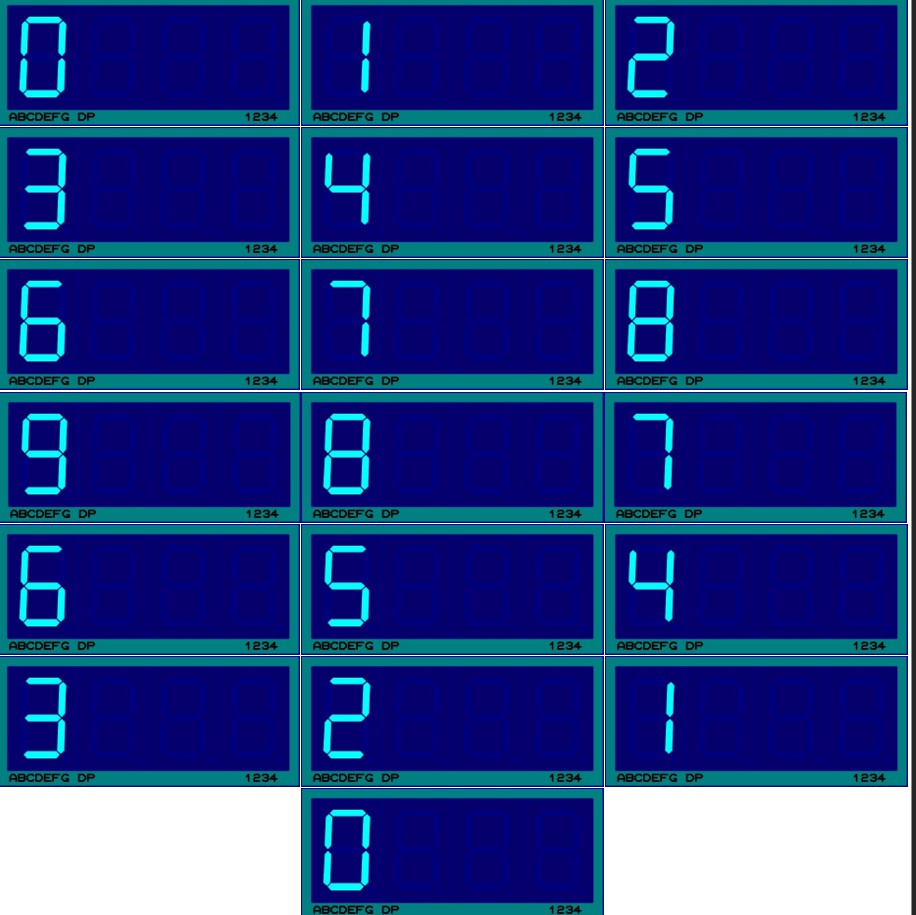
\includegraphics[scale=0.9,cframe=blue 0.5pt 3pt]{./problem 1.jpg}
  \textit{\caption{Proteus output for count 0-9 and back to 0}}
\end{figure}

%%%%%%%%%%%%%%%%%%%%%%%%%%

%%%%%%%%%%%%%%%%%%%%%222222222222222222222

\begin{Q}
  {
    Write a code to design a double digit decimal counter that counts up from 00 to 20 and back to 00 indefinitely.
  }
\end{Q}
\anscode{2}{2.a}{2.c}

\textbf{OUTPUT:}

Here two part of total four 7-segment LEDs is used  to count from 00-20 and them back to 00
\begin{figure}[H]
  \centering
  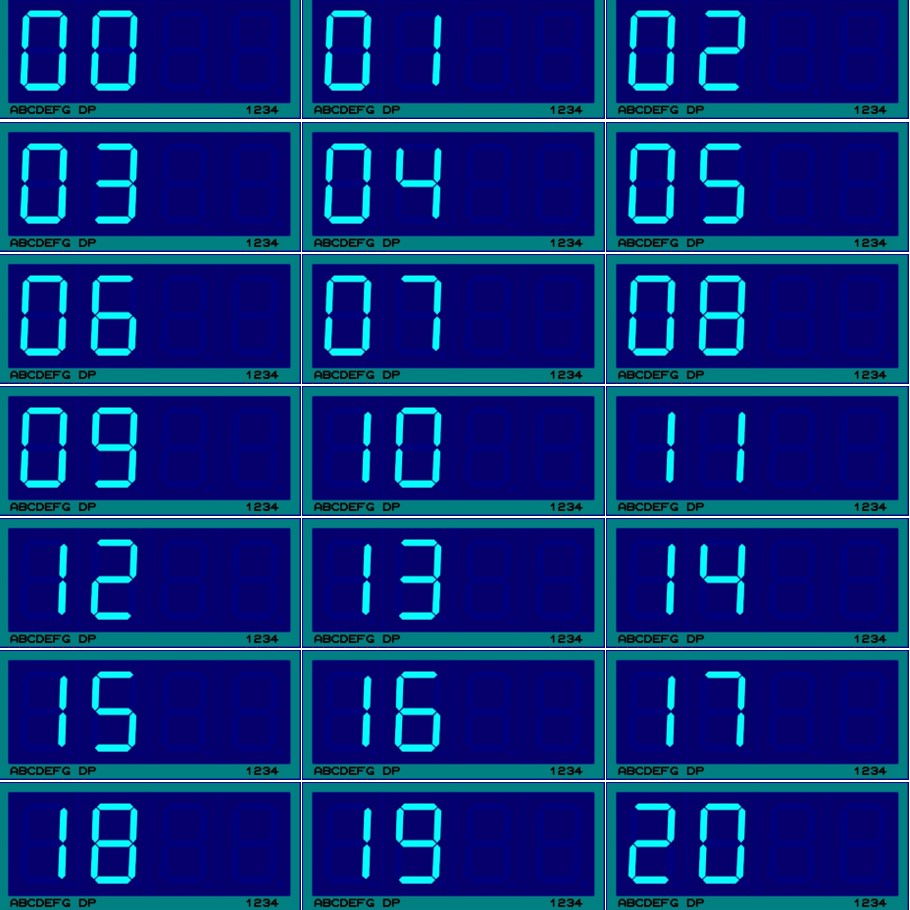
\includegraphics[scale=0.9,cframe=blue 0.5pt 3pt]{./Problem2a.jpg}
  \textit{\caption{Proteus output for count 00-20}}
\end{figure}

\begin{figure}[H]
  \centering
  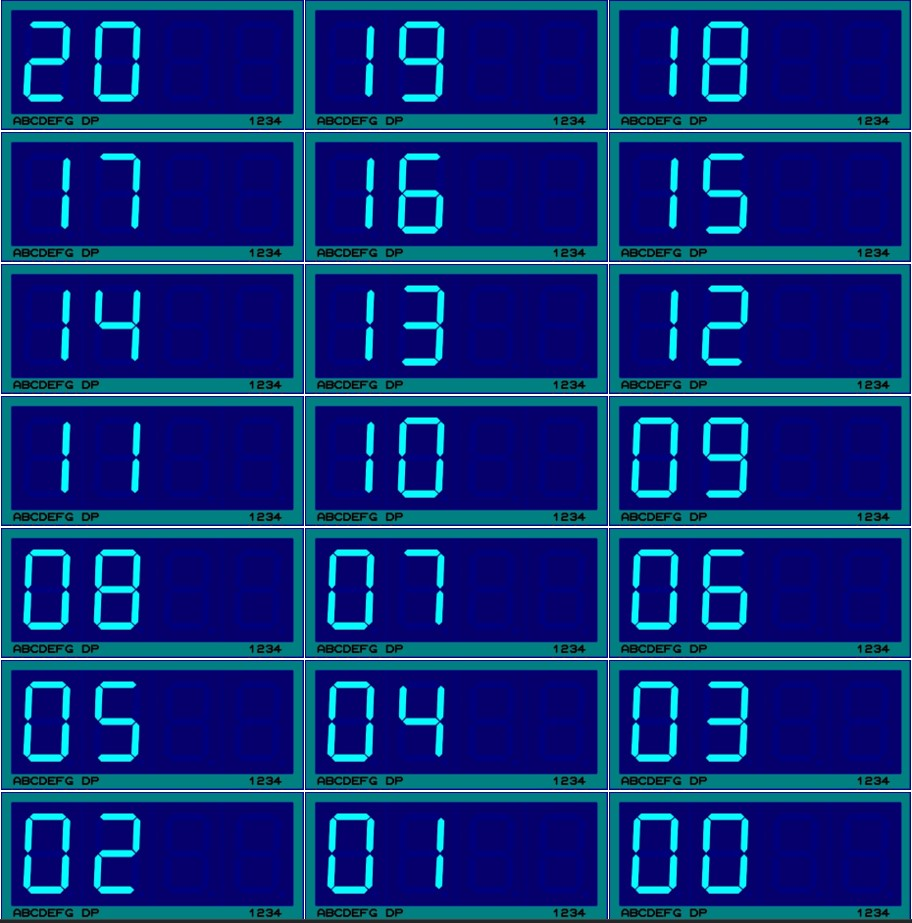
\includegraphics[scale=0.9,cframe=blue 0.5pt 3pt]{./problem2b.jpg}
  \textit{\caption{Proteus output for count 20-00}}
\end{figure}
%%%%%%%%%%%%%%%%%%%%%%%

%%%%%%%%%%%%%%%%333333333333333333
\begin{Q}
  {
    Write a code to display the first (N) numbers of the Fibonacci sequence, where the number (N) must be stored in a memory location and can be any integer from 1 to 10.The sequence should repeat indefinitely.
  }
\end{Q}
\enlargethispage{\baselineskip}
\anscode{3}{3.a}{3.c}

\textbf{OUTPUT:}

Fibonacci sequence of first 8 numbers is shown  below:

\begin{figure}[H]
  \centering
  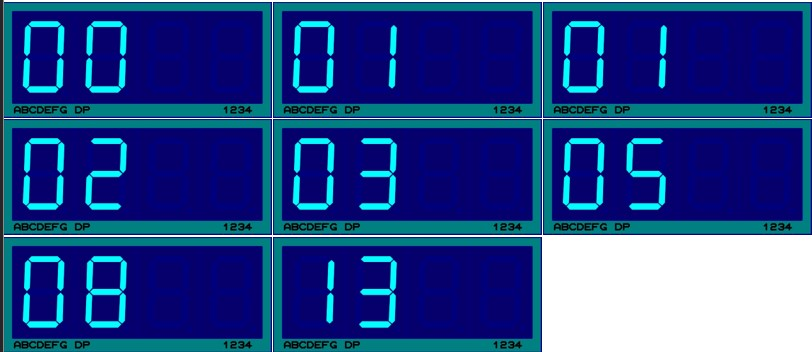
\includegraphics[scale=1,cframe=blue 0.5pt 3pt]{./problem 3.jpg}
  \textit{\caption{Proteus output Fibonacci sequence of first 8 numbers}}
\end{figure}
%%%%%%%%%%%%%%%%%%%%%%%

%%%%%%%%%%%%%%%%%4444444444444444444444
\begin{Q}
  {
    Write a code to generate the multiplication table of a number (N) stored in a memory location which can be any integer from 1 to 10.
    Repeat the sequence indefinitely.
  }
\end{Q}
\anscode{4}{4.a}{4.c}
\textbf{OUTPUT:}

Multiplication table for 7 is shown below

\begin{figure}[H]
  \centering
  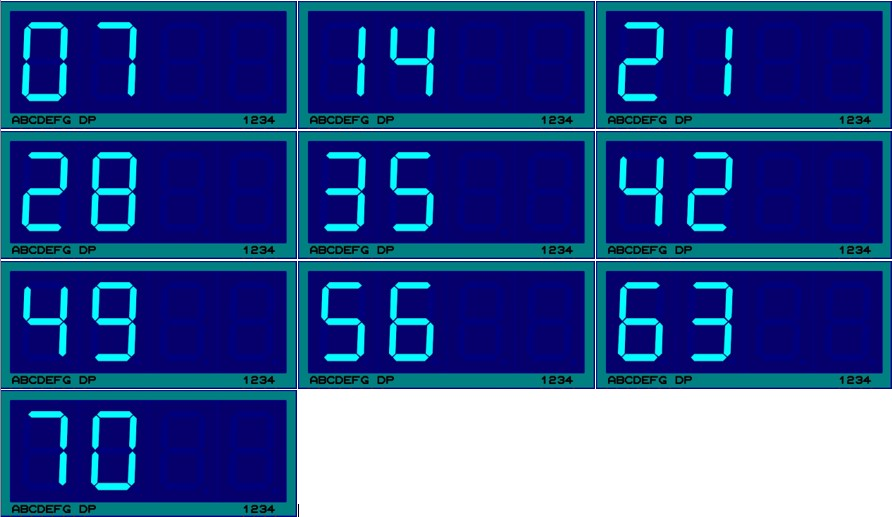
\includegraphics[scale=0.8,cframe=blue 0.5pt 3pt]{./problem 4.jpg}
  \textit{\caption{Proteus output for Multiplication table of 7}}
\end{figure}

%%%%%%%%%%%%%%%%%%%%%%%


%%%%%%%%%%%%%%%%%%%%%%%%%%%%%555555555555555555555
\begin{Q}
  {
    Write a code to display the roll numbers of your lab group members one by one in static format.
    Each student roll number should be of four characters.
    Display of student roll numbers should repeat indefinitely.
  }
\end{Q}

\anscode{5}{5.a}{5.c}

\textbf{OUTPUT:}

Here E is used for Electronics and 403 is my class Roll no.

\begin{figure}[H]
  \centering
  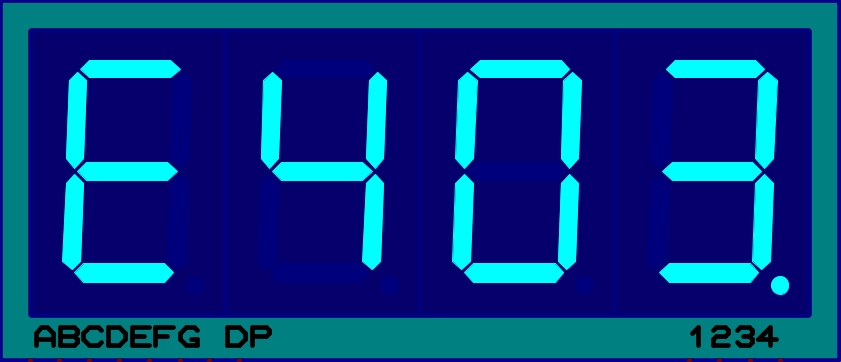
\includegraphics[scale=1.8,cframe=blue 0.5pt 3pt]{./Problem 5.jpg}
  \textit{\caption{Proteus output for Roll no. Display}}
\end{figure}

%%%%%%%%%%%%%%%%%%%%%%%

%%%%%%%%%%%%%%%66666666666666666666
\begin{Q}
  {
    Write a code to display the roll numbers of your lab group members in scrolling format, separated by using decimal point.
    Roll numbers should be scrolled towards the left and is repeated indefinitely.
  }
\end{Q}

\anscode{6}{6.a}{6.c}
\textbf{OUTPUT:}

My Roll no. E403. is Shown in scrolling Format and scrolling toward left.

\begin{figure}[H]
  \centering
  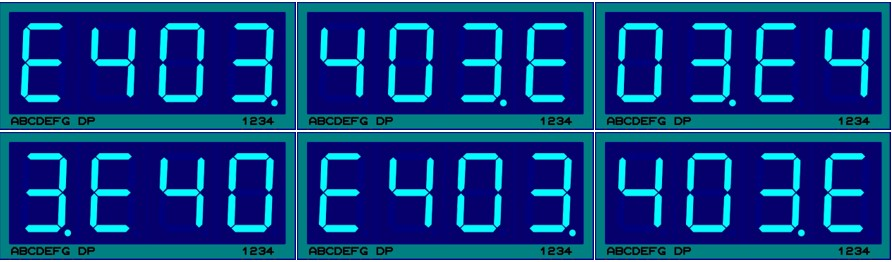
\includegraphics[scale=0.9,cframe=blue 0.5pt 3pt]{./problem 6.jpg}
  \textit{\caption{Proteus output for Scrolling roll no.}}
\end{figure}

%%%%%%%%%%%%%%%%%%%%%%%

\pagebreak

\section{Discussion and Conclusion}

In this Experiment , we familiarize ourself with seven segment display and its operation through 8051 microcontroller.
We performed single digit count, double digit count, generate Multiplication Table, Fibonacci sequence and scrolling effect  of certain number.
we used both Assembly and C language approach to achieve the above  task.



\end{document}